\documentclass[11pt,a4paper]{article}
\usepackage{amsmath}
\usepackage{amssymb}
\usepackage{graphicx}
\usepackage{color}
\usepackage{fancyhdr}
\usepackage[margin=3.5cm]{geometry}
\usepackage{framed}
\usepackage{enumerate}
\usepackage{textcomp}
\usepackage{fancyvrb}

\usepackage[colorlinks=true,urlcolor=blue,citecolor=black,linkcolor=black]{hyperref}
\def\ket#1{\left|#1\right\rangle}
\def\bra#1{\left\langle#1\right|}
\def\braket#1{\left\langle#1\right\rangle}

\fancyhf{}
\lhead{NTU/SPMS/PH2198--PH2199 Lab}
\rhead{Error Analysis}
\lfoot{\tiny\textcopyright \;2018 Nanyang Technological University.  Released under \href{http://creativecommons.org/licenses/by-sa/4.0/}{CC BY-SA 4.0}.}
\rfoot{\thepage}
\pagestyle{fancy}

\definecolor{dgreen}{RGB}{70,128,13}

\begin{document}

\begin{center}
\textbf{Division of Physics\;\,\&\;Applied Physics}

\textbf{PH2198/2198---Physics Laboratory IIA/IIB}

\vskip 0.05in

\underline{\LARGE Error Analysis}
\end{center}

\section{Measurement error}

The result of a single measurement should be reported in the format
\begin{equation*}
  (\textrm{estimate})\, \pm\, (\textrm{measurement error}).
\end{equation*}
The \textbf{estimate} is your best guess for the true value, while the
\textbf{measurement error} states the range where the true value might
lie.  By convention, the estimate and measurement error are formatted
according to the these rules \cite{Hughes}:
\begin{enumerate}
\item 
  The measurement error has \underline{one significant figure}.

\item
  The estimate has the same precision as the measurement error.
\end{enumerate}

\noindent
Suppose you use a digital multimeter to measure the current in a
circuit, and the readout is stable (i.e., not fluctuating).  Then you
should report a result like this:
\begin{center}
\raisebox{-.4\height}{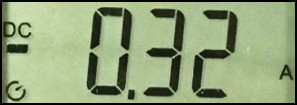
\includegraphics[width=0.23\textwidth]{readout.jpg}}
$\;\;=\; \left(0.320 \pm 0.005\right) \, \mathrm{A}$
\end{center}
Why?  According to the readout, the value is between
$0.315\,\mathrm{A}$ (rounded up to $0.32\,\mathrm{A}$) and
$0.324999\dots\mathrm{A}$ (which is rounded down).  So the measurement
error is $\pm 0.005 \, \mathrm{A}$.  Note that the estimate is
reported as $0.320 \,\mathrm{A}$ to have the same precision as the
error.

When using a device with hatch marks, such as a ruler or analog
oscilloscope display, the measurement error is determined by the
smallest markings.  For example, if the smallest markings on a ruler
have $1\,\mathrm{mm}$ spacing, the measurement error is $\pm 0.5
\,\textrm{mm}$, so a reading should be reported like this:
\begin{center}
\raisebox{-.4\height}{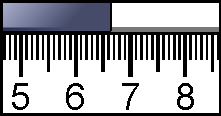
\includegraphics[width=0.23\textwidth]{ruler.pdf}}
$\;\;=\; \left(6.60 \pm 0.05\right) \, \mathrm{cm}$
\end{center}

In more complicated situations, you must exercise your judgment.  For
instance, suppose you have a digital multimeter reading that is not
stable: the last digit changes constantly, so that the reading
fluctuates between $0.32$, $0.33$, and $0.34\,\mathrm{A}$.  The value
is between $0.315\,\mathrm{A}$ and $0.344999\dots\mathrm{A}$, which is
a range of $\pm0.015\,\mathrm{A}$.  Since we use one significant
figure for errors, the result is reported like this:
\begin{center}
\raisebox{-.4\height}{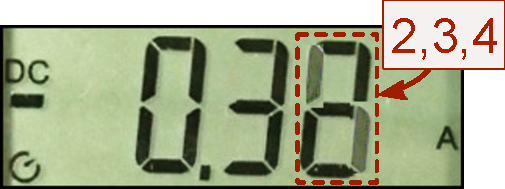
\includegraphics[width=0.23\textwidth]{readout2.pdf}}
$\;\;=\; \left(0.33 \pm 0.02\right) \, \mathrm{A}$
\end{center}
Alternatively, suppose the last digit is changing so fast that you
can't make out its values at all.  Then you can report the result like
this:
\begin{center}
\raisebox{-.4\height}{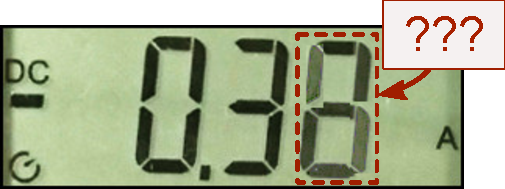
\includegraphics[width=0.25\textwidth]{readout3.pdf}}
$\;\;=\; \left(0.35 \pm 0.05\right) \, \mathrm{A}$
\end{center}

Measurement uncertainties can also come from other aspects of an
experiment.  Suppose you use a ruler to measure the distance to an
object, but the object wobbles by $\pm 2\,\textrm{mm}$, larger than
the $1\,\textrm{mm}$ hatch marks of the ruler.  In that case, you should
report a measurement error of $\pm 2\,\textrm{mm}$, not $\pm
0.05\,\textrm{mm}$.

\section{Sampling Error (Repeated Measurements)}

In some experiments, the system being measured is intrinsically
random.  For example, radioactive decay occurs randomly, so counting
the number of decay events yields a slightly different result from
interval to interval, \textit{no matter how precise your apparatus
  is}.  Often, we find a \textbf{mean} value by taking many
measurements and averaging them.  The result is reported in the format
\begin{equation*}
  \textrm{(estimated mean)} \,\pm\, \textrm{(standard error of the mean)}.
\end{equation*}
The quantity after the $\pm$ refers to \textbf{sampling error}, which
is \textit{not} the same as measurement error.  Sampling error arises
because you only took a finite number of samples, so your estimate of
the mean is not completely certain.

In this type of scenario, measurement error is usually ignored, as the
sampling error caused by the system's randomness is larger than the
measurement error.  (In the opposite case, where measurement error is
larger, there'd be no point doing repeated measurements.  And if the
measurement error is about as large as the system's randomness, you're
probably doing social science, so good luck with that.)

Suppose you take $N$ measurements, and the results are $X_1, X_2,
\dots, X_N$.  Then
\begin{equation*}
  \textrm{estimated mean} \equiv \bar{X} = \frac{X_1 + X_2 + \cdots + X_N}{N}.
\end{equation*}
You can compute $\bar{X}$ using the \texttt{mean} function in
\href{https://docs.scipy.org/doc/numpy/reference/generated/numpy.mean.html}{Python}
or \href{https://www.mathworks.com/help/matlab/ref/mean.html}{Matlab}.
Also,
\begin{equation*}
  \textrm{standard error of the mean} = \frac{\sigma}{\sqrt{N}},
\end{equation*}
where $\sigma$ is the \textbf{standard deviation of the sample},
defined as
\begin{equation*}
  \sigma = \sqrt{\frac{\sum_{n=1}^N(X_n-\bar{X})^2}{N-1}}.
\end{equation*}
You can compute $\sigma$ using the \texttt{std} function in
\href{https://docs.scipy.org/doc/numpy/reference/generated/numpy.std.html}{Python}
or \href{https://www.mathworks.com/help/matlab/ref/std.html}{Matlab}.

\section{Error Estimates for Sums, Products, and Powers}
\label{sec:propagation}

When analyzing experiments, you often need to take sums, products, and
powers of measured data.  For instance, you might measure the voltage
$V$ and current $I$ across a circuit, and use them to find the
resistance $R = V/I$.  Errors in $V$ and $I$ will turn into errors in
$R$.  This is called \textbf{error propagation}.

The basic rules of error propagation are easy to summarize (if you
want the detailed derivations, refer to Ref.~\cite{Hughes}).  Consider
two independent quantities $X \pm \Delta X$ and $Y \pm \Delta Y$.  We
call $\pm\Delta X$ and $\pm \Delta Y$ the \textbf{standard errors} for
$X$ and $Y$, regardless of whether they originate from measurement
error or sampling error.  Now, suppose we derive $Z \pm \Delta Z$ by
addition or subtraction of $X$ and $Y$:
\begin{equation*}
  \left\{\begin{array}{l}Z = X + Y \;\;\mathrm{or}\\ Z = X - Y
  \end{array}  \right. \;\;\; \leftrightarrow \;\;\; \Delta Z = \sqrt{(\Delta X)^2 + (\Delta Y)^2}.
\end{equation*}
More generally, for any two (error-free) constants $\alpha$ and $\beta$,
\begin{equation*}
  \;\;\qquad Z = \alpha X + \beta Y \qquad \leftrightarrow \;\;\; \Delta Z = \sqrt{\alpha^2(\Delta X)^2 + \beta^2 (\Delta Y)^2}.
\end{equation*}
For products and fractions,
\begin{equation*}
  \quad\qquad\;\left\{\begin{array}{l}Z = \alpha XY \;\;\mathrm{or}\\ Z = \alpha X/Y
  \end{array}  \right. \quad \leftrightarrow \;\;\;
  \frac{\Delta Z}{|Z|} = \sqrt{\left(\frac{\Delta X}{X}\right)^2 + \left(\frac{\Delta Y}{Y}\right)^2}.
\end{equation*}
For powers, exponentials and logarithms,
\begin{align}
  \begin{aligned}
  Z &= X^n \quad\qquad\; \leftrightarrow \;\;\; \frac{\Delta Z}{|Z|} = |n| \,\frac{\Delta X}{|X|} \\
    Z &= \ln(X) \qquad\, \leftrightarrow \;\;\; \Delta Z \,= \frac{\Delta X}{|X|} \\
    Z &= \log_{10}(X) \;\;\; \leftrightarrow \;\;\; \Delta Z \, = \frac{1}{\ln(10)} \, \frac{\Delta X}{|X|} \\
    Z &= \exp(\alpha X) \;\;\; \leftrightarrow \;\;\; \frac{\Delta Z}{|Z|} = |\alpha|\,\Delta X.
  \end{aligned} \nonumber
\end{align}

More complicated formulas can usually be handled by combining these
rules.  For example, suppose you seek an object's kinetic energy $T =
\frac{1}{2}mv^2$, using data $m \pm \Delta m$ and $v \pm \Delta v$.
First, find the error in the quantity $v^2$ using the rule for powers:
\begin{equation*}
  \frac{\Delta (v^2)}{|v^2|} = 2 \frac{\Delta v}{|v|}.
\end{equation*}
Then, plug this into the rule for products:
\begin{align}
  \begin{aligned}
    \Delta T &= |T|\, \sqrt{\left(\frac{\Delta m}{m}\right)^2
      + \left(\frac{\Delta (v^2)}{v^2}\right)^2} \\
    &= \frac{1}{2} m v^2\, \sqrt{\left(\frac{\Delta m}{m}\right)^2
      + 4 \left(\frac{\Delta v}{v}\right)^2}.
  \end{aligned} \nonumber
\end{align}

\section{Curve Fitting}
\label{sec:curvefit}

Many experiments require you to perform \textbf{curve fitting}.  You
have data points
\begin{equation*}
  \begin{array}{c}X_1 \\ X_2 \\ \vdots \\ X_N \end{array}
  \begin{array}{c}Y_1 \\ Y_2 \\ \vdots \\ Y_N \end{array}
\end{equation*}
which may be either direct measurement results, or derived from
measurements.  You are then required to fit these data to a relation
such as
\begin{equation*}
  Y = b_0 + b_1 X.
\end{equation*}
The goal is to determine $b_0$ and $b_1$, which are called
\textbf{estimators}.

Curve fitting, and the propagation of error into estimators, is a
complicated subject within the mathematical discipline of statistics.
For most experiments in this course, you will only need the most basic
method, which is called \textbf{weighted linear least squares
  regression}.

In this method, each data point $(X_i,Y_i)$ is assigned a relative
weight $w_i$.  Data points with smaller errors are considered more
important (i.e., they have more ``weight'').  A standard weight
assignment is
\begin{equation*}
  w_i = \frac{1}{\Delta Y_i^{2}}.
  \label{weighting}
\end{equation*}
Note that this ignores the errors in $X$.  There is no standard
weighting procedure that accounts for errors in both $X$ and $Y$.  So
you should let the variable with more ``relevant'' error be the $Y$
variable, so its error is used for the curve-fitting weights.

As an example, suppose we measure the period of a pendulum, $T$, with
varying arm length $L$.  Theoretically, $T$ and $L$ are related to the
gravitational constant $g$ by
\begin{equation*}
  T = 2\pi \sqrt{\frac{L}{g}} \;\;\; \Rightarrow \;\;\; T^2 = \frac{4\pi^2}{g} \, L.
\end{equation*}
We can fit our data to the relation
\begin{equation*}
  T^2 = b_0 + b_1 L,
\end{equation*}
and use $b_1$ to estimate $4\pi^2/g$.  Hence, we can find $g =
4\pi^2/b_1$, and its error $\Delta g$:
\begin{equation*}
  \frac{\Delta g}{g} = \frac{\Delta b_1}{b_1} \;\;\;\Rightarrow\;\;\;
  \Delta g = \frac{4\pi^2\Delta b_1}{b_1^2}.
\end{equation*}
Suppose all our measurements of $T$ have the same measurement error
$\pm \Delta T$.  From the error propagation rule for powers
(Section~\ref{sec:propagation}),
\begin{equation*}
  \frac{\Delta (T^2)}{T^2} = 2 \frac{\Delta T}{T} \;\;\;\Rightarrow
  \;\;\; \Delta (T^2) = 2\,T\,\Delta T.
\end{equation*}
Thus, the errors in $T^2$ are not uniform: data points with large $T$
have more error.

\subsection{Sample Python program}

A sample Python program for weighted linear least squares curve
fitting is shown below.  The fitting is done by the
\href{https://docs.scipy.org/doc/scipy/reference/generated/scipy.optimize.curve_fit.html}{\texttt{curve\_fit}}
function, from the
\href{https://docs.scipy.org/doc/scipy/reference/optimize.html}{\texttt{scipy.optimize}}
module.

In this program, \texttt{curve\_fit} is called with four inputs: the
model function, the $x$ data, the $y$ data, and the standard errors of
the $y$ data.  The first input is a function that you must define,
telling \texttt{curve\_fit} what kind of curve to fit to (in this
case, a first-order polynomial).  The last three inputs are arrays of
numbers.

The \texttt{curve\_fit} function returns two outputs.  The first
output is an array of estimators (i.e., the additional inputs that,
when passed to the model function, give the best fit to the data).
The second output is a ``covariance matrix'', whose diagonal terms are
the estimator variances (i.e., taking their square roots yields the
standard errors of the estimators).

\begin{Verbatim}[frame=single,baselinestretch=1,fontsize=\small,commandchars=\\\{\}]
from scipy import *
from scipy.optimize import curve_fit

\textcolor{dgreen}{## Input data (generated by simulation with random noise).}
L  = array([0.10, 0.16, 0.22, 0.28, 0.34, 0.40, 0.46, 0.52, 0.58, 0.64])
dL = array([0.01, 0.01, 0.01, 0.01, 0.01, 0.01, 0.01, 0.01, 0.01, 0.01])
T  = array([0.71, 0.76, 0.91, 1.00, 1.20, 1.14, 1.44, 1.40, 1.53, 1.58])
dT = array([0.05, 0.05, 0.05, 0.05, 0.05, 0.05, 0.05, 0.05, 0.05, 0.05])

Tsq = T**2           \textcolor{dgreen}{# Estimates for T^2}
Tsq_error = 2*T*dT   \textcolor{dgreen}{# Errors for T^2, from error propagation rules}

\textcolor{dgreen}{## Define an order-1 polynomial function, and use it to fit the data.}
def f(x, b0, b1): return b0 + b1*x
est, covar = curve_fit(f, L, Tsq, sigma=Tsq_error)

\textcolor{dgreen}{## Estimators and their errors:}
b0, b1 = est               \textcolor{dgreen}{# Estimates of intercept and slope}
db0 = sqrt(covar[0,0])     \textcolor{dgreen}{# Standard error of intercept}
db1 = sqrt(covar[1,1])     \textcolor{dgreen}{# Standard error of slope}

g  = 4*pi*pi/b1            \textcolor{dgreen}{# Estimate for g (computed from b1)}
dg = (g/b1)*db1            \textcolor{dgreen}{# Estimate for standard error of g}

\textcolor{dgreen}{## Plot the data points, with error bars}
import matplotlib.pyplot as plt
plt.errorbar(L, Tsq, xerr=dL, yerr=Tsq_error, fmt='o')
plt.xlabel('Pendulum length L (m)', fontsize=12)
plt.ylabel('Squared period T^2 (s^2)', fontsize=12)
\textcolor{dgreen}{## Include the fitted curve in the plot}
L2 = linspace(0, 0.7, 100)
plt.plot(L2, b0 + b1*L2)
\textcolor{dgreen}{## State fitted value of g in the figure title}
plt.title("g = \{:.1f\} +/- \{:.1f\} m/s^2".format(g, dg), fontsize=12)
plt.show()
\end{Verbatim}
The resulting plot looks like this:
\begin{center}
  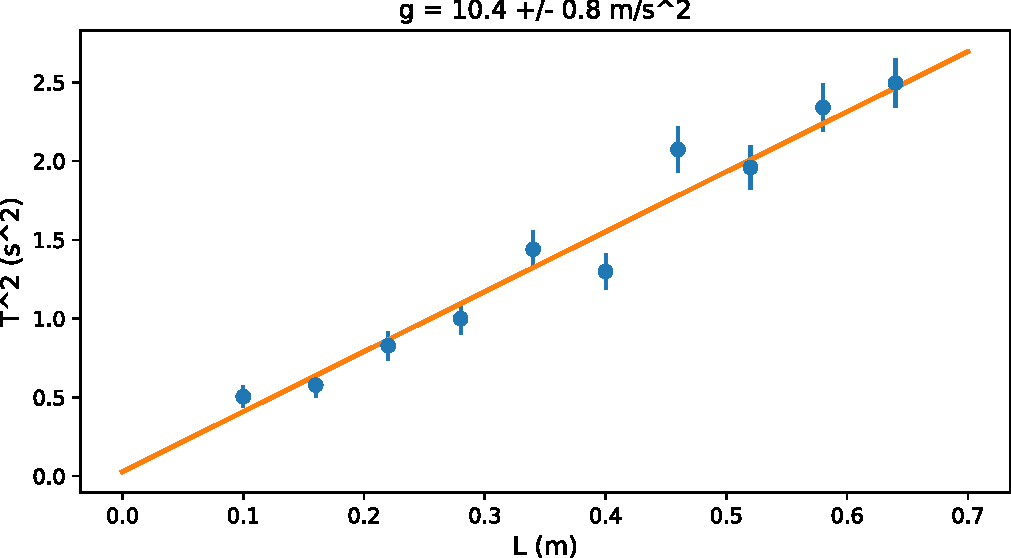
\includegraphics[width=0.8\textwidth]{errorpy.pdf}
\end{center}

\subsection{Sample Matlab program}

Here is a sample Matlab program for weighted linear least squares
curve fitting.  It uses the
\href{https://www.mathworks.com/help/stats/glmfit.html}{\texttt{glmfit}}
function from Matlab's
\href{https://www.mathworks.com/help/stats/index.html}{Statistics
  Toolbox}.

\begin{Verbatim}[frame=single,baselinestretch=1,fontsize=\small,commandchars=\\\{\}]
L  = [0.10, 0.16, 0.22, 0.28, 0.34, 0.40, 0.46, 0.52, 0.58, 0.64];
dL = [0.01, 0.01, 0.01, 0.01, 0.01, 0.01, 0.01, 0.01, 0.01, 0.01];
T  = [0.71, 0.76, 0.91, 1.00, 1.20, 1.14, 1.44, 1.40, 1.53, 1.58];
dT = [0.05, 0.05, 0.05, 0.05, 0.05, 0.05, 0.05, 0.05, 0.05, 0.05];

Tsq = T.^2;            \textcolor{dgreen}{% Estimates for T^2}
Tsq_error = 2*T.*dT;   \textcolor{dgreen}{% Errors for T^2, from error propagation rules}

\textcolor{dgreen}{%% Fit L and Tsq with weighted linear least squares}
wt = 1 ./ (Tsq_error.^2);   \textcolor{dgreen}{% Vector of weights}
[est, dev, stats] = glmfit(L, Tsq, 'normal', 'weights', wt);

\textcolor{dgreen}{%% Estimators and their errors:}
b0  = est(1);                \textcolor{dgreen}{% Estimate of intercept}
b1  = est(2);                \textcolor{dgreen}{% Estimate of slope}
db0 = stats.se(1);           \textcolor{dgreen}{% Standard error of intercept}
db1 = stats.se(2);           \textcolor{dgreen}{% Standard error of slope}

g  = 4*pi*pi/b1;              \textcolor{dgreen}{% Estimate for g (computed from b1)}
dg = (g/b1)*db1;              \textcolor{dgreen}{% Estimate for standard error of g}

\textcolor{dgreen}{%% Plot the data points and fitted curve}
errorbar(L, Tsq, Tsq_error, Tsq_error, dL, dL, "o");
xlabel("Pendulum length L (m)");
ylabel("Squared period T^2 (s^2)");
\textcolor{dgreen}{%% State the fitted value of g in the figure}
title(sprintf("g = %.1f +/- %.1f m/s^2", g, dg));
\textcolor{dgreen}{%% Plot the fitted curve}
L2 = linspace(0, 0.7, 100);
hold on; plot(L2, b0 + b1*L2); hold off;
\end{Verbatim}
The resulting plot looks like this:
\begin{center}
  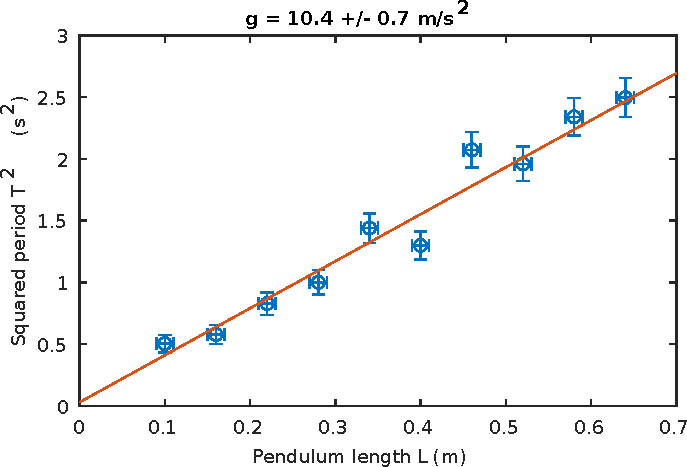
\includegraphics[width=0.73\textwidth]{errormatlab.pdf}
\end{center}

\subsection{Curve fitting with Origin}

The procedure for curve fitting with Origin is summarized below.
For more details, consult the
\href{https://www.originlab.com/doc/Origin-Help/Linear-Polynomial-Regression}{Origin
  online documentation}.

\begin{enumerate}
\item Populate a worksheet with columns for (i) $X$, (ii) $Y$, and
  (iii) $\Delta Y$.  You can enter the numbers manually, or import
  them from an external file.

\item Select the menu item
  \texttt{Plot$\,\rightarrow\,$Symbol$\,\rightarrow\,$Scatter}.  Click on the
  appropriate boxes to specify (i) which column to use for the
  horizontal ($X$) variable, (ii) which column to use for the vertical
  ($Y$) variable, and (iii) which column to use for the error $\Delta
  Y$.

\item Select the menu item
  \texttt{Analysis$\,\rightarrow\,$Fitting$\,\rightarrow\,$Linear
    Fit}.  In the dialog box, check that the right fitting options are
  entered.  Under \texttt{Fit Control$\,\rightarrow\,$Errors as
    Weight}, ensure that the \texttt{Instrumental} option is chosen.
  This corresponds to the standard weighting scheme from
  Section~\ref{sec:curvefit}.  Once ready, perform the fit.

\item The fitted curve will be inserted automatically into the graph.
  By default, a \texttt{Fit Results} table is also automatically
  added; you can click-and-drag to move or resize this table, and
  double-click to edit its contents.

  By default, Origin makes the table too small to be legible, so you
  ought to increase the size.  Also, you should omit any statistical
  quantities listed in this table that are not relevant to your data
  analysis (e.g., the Pearson's $r$).  Finally, you still need to
  convert the estimators into whatever quantities you are ultimately
  interested in (such as $g$).
\end{enumerate}

The resulting plot looks like this:
\begin{center}
  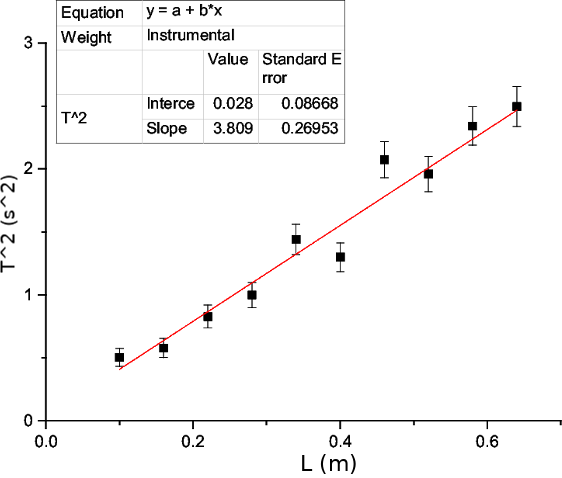
\includegraphics[width=0.56\textwidth]{origin.png}
\end{center}


\begin{thebibliography}{99}
\bibitem{Hughes} I.~G.~Hughes and T.~P.~A.~Hase, \textit{Measurements
  and their uncertainties} (Oxford University Press, 2010).
\end{thebibliography}

\end{document}
